\documentclass[10pt,twocolumn,a4paper]{article}

% Layout retained from the supplied Phase II report.
\usepackage[top=1in,bottom=1in,left=0.75in,right=0.75in,columnsep=0.25in]{geometry}
\usepackage[T1]{fontenc}
\usepackage[utf8]{inputenc}
\usepackage{cite}
\usepackage{amsmath,amssymb}
\usepackage{array,booktabs,tabularx,multirow,makecell}
\usepackage{setspace,parskip,titlesec,xcolor,abstract,graphicx,enumitem,adjustbox,caption}
\usepackage{tikz}
\usetikzlibrary{arrows.meta,positioning,shapes,fit,backgrounds,calc}
\usepackage{hyperref}
\hypersetup{colorlinks=true,linkcolor=black,citecolor=blue,urlcolor=blue,
  pdftitle={ZKP-Authorized Homomorphic Matching and Auditable Record Revocation for Organ Donation},
  pdfauthor={Chirag Parmar}}
\titleformat{\section}{\normalfont\normalsize\bfseries\scshape}{\Roman{section}.}{0.5em}{}
\titleformat{\subsection}{\normalfont\normalsize\itshape}{\Alph{subsection}.}{0.5em}{}
\titlespacing*{\section}{0pt}{6pt}{3pt}
\titlespacing*{\subsection}{0pt}{4pt}{2pt}
\renewcommand{\abstractnamefont}{\normalfont\bfseries}
\renewcommand{\abstracttextfont}{\normalfont\small}
\setlength{\absleftindent}{0pt}
\setlength{\absrightindent}{0pt}
\setlength{\textfloatsep}{8pt plus 2pt minus 2pt}
\setlength{\floatsep}{6pt plus 2pt minus 2pt}
\setlength{\intextsep}{7pt plus 2pt minus 2pt}
\setlength{\dbltextfloatsep}{8pt plus 2pt minus 2pt}
\setlength{\dblfloatsep}{7pt plus 2pt minus 2pt}
\captionsetup{font=small,labelfont=bf,skip=4pt}
\definecolor{novelty}{RGB}{0,100,60}
\definecolor{proposed}{RGB}{100,60,0}
\setlist{leftmargin=*,nosep}
\setlength{\emergencystretch}{1em}
\newcommand{\code}[1]{\texttt{#1}}
\newcommand{\CurrentTestsPassed}{35}
\newcommand{\CurrentTestsSkipped}{1}
\newcommand{\ProofMedianMs}{2,922.25}
\newcommand{\EvaluationMedianMs}{230.73}
\newcommand{\VerificationMedianGas}{310,463}


\title{\large\textbf{ZKP-Authorized Homomorphic Matching and Auditable Record Revocation for Organ Donation}}
\author{\normalsize Chirag Parmar\\
  \small M250738CS\\[2pt]
  \normalsize Guided by: Dr.~Abidha V.P \& Dr.~Bijoy Das\\
  \small Department of Computer Science and Engineering, NIT Calicut}
\date{Major Project, Phase II --- October 2026}

\begin{document}
\raggedbottom
\maketitle
\thispagestyle{empty}

\begin{abstract}
\noindent
Organ-donation information systems require approved participant access, confidential
record processing and an auditable record lifecycle. This report presents a local,
synthetic research prototype combining administrator-approved role membership,
browser-generated Groth16 proofs, BFV homomorphic evaluation, AES-wrapped IPFS
storage and recoverable record revocation. A depth-20 Poseidon membership circuit
binds authorization to a wallet, chain, issuer and membership-root version. The
backend is explicitly trusted to receive registration inputs, encrypt records and
decrypt permitted calculation results; no function-specific functional-encryption
keys are implemented. The revised chain stores opaque identifiers, content anchors
and lifecycle metadata rather than plaintext clinical attributes. A fixed synthetic
policy separates ABO eligibility from six binary tissue features and recipient
urgency. The recorded complete validation run passed 28 tests with no skips and
11 live browser checks. A subsequent regression run passed \CurrentTestsPassed{}
tests with \CurrentTestsSkipped{} explicitly skipped infrastructure test. Dedicated
experiments use ten warmups and thirty measured repetitions: median Node proving
time is \ProofMedianMs{}\,ms, BFV evaluation is \EvaluationMedianMs{}\,ms and warmed
proof verification plus authorization uses \VerificationMedianGas{} gas.
These findings establish behavior and local implementation costs under stated
assumptions, not clinical validity, participant anonymity, universal erasure or
regulatory compliance.

\smallskip\noindent
\textbf{Keywords:} Organ donation; zero-knowledge proofs; role authorization;
BFV homomorphic encryption; IPFS; encrypted records; recoverable revocation.
\end{abstract}

\section{Introduction}
\label{sec:introduction}

An organ-donation workflow involves participants with different responsibilities,
sensitive records and decisions that need a clear audit trail. A shared ledger can
record who registered or retired a record, but ledger transparency does not provide
confidentiality. Equally, encrypting stored data does not establish that a caller
has an institutionally approved role. Access authorization, confidential storage,
computation and lifecycle recovery must therefore be treated as separate mechanisms.

This Phase~II work evaluates their integration in a deliberately bounded prototype.
The system uses a local Hardhat development chain, synthetic donor and recipient
records, browser-side proof generation and one trusted BFV service. It does not
implement hospital governance, transport confirmation, transplant execution or
clinical allocation. Public deployment and real patient data are outside the
evaluated scope.

In the implemented protocol, a ZKP establishes approved role membership and
authorizes a session. A trusted service owns a general BFV decryption key and
releases results from a fixed function. Revocation deactivates canonical records
and completes defined local cleanup. External copies and historical outputs remain
outside that guarantee.

The resulting contributions are:
\begin{enumerate}
\item An approved-enrollment protocol with browser-held credentials, wallet-bound
membership proofs, root-version checks and signed API sessions.
\item A reproducible synthetic matching model evaluated under BFV, with explicit
eligibility, encoding, integer bounds and output restrictions.
\item Encrypted off-chain storage with persistent encrypted keys, canonical
record mappings and recoverable cleanup for donors and recipients.
\item Authorization, arithmetic, recovery and browser evidence, together with
stage-specific gas and timing measurements.
\end{enumerate}
The contribution is an evaluated integration rather than a new cryptographic
primitive or a verified claim of being the first such system.

\section{Literature Review}
\label{sec:litreview}

\subsection{Blockchain-Based Organ Donation Management}
Hawashin et al.~\cite{hawashin} study blockchain-based management for organ donation
and transplantation. Their Ethereum workflow illustrates the value of stakeholder
permissions and lifecycle provenance. This report uses an organ-donation setting
but implements a narrower set of registration, matching and revocation operations.
Auditability and confidential computation are evaluated separately rather than
assuming that a blockchain supplies both.

\subsection{Functional and Homomorphic Encryption}
Functional encryption provides function-dependent decryption capabilities~\cite{fe}.
Homomorphic encryption instead supports evaluation over ciphertexts; possession of
a general secret key remains a separate trust issue. BFV supports exact integer
arithmetic, making it suitable for the bounded polynomial used here~\cite{bfv}.
Microsoft SEAL supplies the underlying implementation and parameter-validation
mechanisms~\cite{seal}. A server that controls BFV encryption and decryption is not
thereby an FE construction. This distinction determines the confidentiality claims
and trusted-service assumptions of the present prototype.

\subsection{Encrypted Healthcare Records and Off-Chain Storage}
Vanin et al.~\cite{vanin} investigate personal-health-record protection combining
blockchain, homomorphic encryption and distributed off-chain storage. Their work
provides prior evidence that encrypted computation and healthcare storage can be
integrated. The present study focuses on approved enrollment, constrained result
release and restart/revocation recovery. It does not claim a new general solution
for encrypted healthcare databases or population-scale performance.

\subsection{Zero-Knowledge Membership Authentication}
Groth16 provides succinct pairing-based non-interactive arguments with a
circuit-specific setup~\cite{groth}. Poseidon is designed for efficient arithmetic
circuits and is used for role commitments and Merkle paths~\cite{poseidon}.
Proof soundness concerns satisfaction of the circuit; it does not establish that
an administrator correctly checked a participant's institutional role. In this
implementation, enrollment correctness is a separate trust assumption and wallet
activity remains publicly linkable.

\subsection{Related Integration: Block-Privacy}
Egala, Pradhan and Gupta's Block-Privacy combines blockchain, IPFS, zero-knowledge
protocols and functional encryption for smart healthcare~\cite{egala}. The publisher
records a 2024 proceedings citation with first-online publication in October 2023.
This prior integration precludes an unsupported first-system claim. The present
prototype evaluates approved role sessions, fixed BFV scoring and local recovery;
it does not assert the absence of unexamined features in that work.

Table~\ref{tab:related} summarizes supported positioning. Unverified entries and
placeholder-author references from the old bibliography are retained in the
repository's original-source archive rather than presented as verified evidence.
The older Samsukha comparison requires inspection of the original publication
before its algorithms or reported measurements can support a feature comparison.

\begin{table*}[t]
\centering
\caption{Positioning based on inspected primary sources. A capability not established here is not classified as absent from the original work.}
\label{tab:related}
\scriptsize\renewcommand{\arraystretch}{1.13}
\begin{tabularx}{\textwidth}{>{\raggedright\arraybackslash}p{2.4cm} >{\raggedright\arraybackslash}X >{\raggedright\arraybackslash}X >{\raggedright\arraybackslash}X}
\toprule
Work & Reported focus & Relevance & Boundary of this comparison\\\midrule
Hawashin et al.~\cite{hawashin} & Organ-donation and transplantation management using blockchain & Role-controlled workflow and lifecycle provenance & No claim of clinical or privacy equivalence\\
Vanin et al.~\cite{vanin} & Blockchain, HE and off-chain personal-health-record sharing & Encrypted healthcare storage and computation & Its workload is not the synthetic matching workload measured here\\
Block-Privacy~\cite{egala} & Blockchain, IPFS, ZK protocols and FE for smart healthcare & Prior integration of relevant mechanisms & Unexamined implementation details are not marked missing\\
This prototype & Approved role sessions, fixed BFV matching and recoverable local revocation & Code-linked tests and local stage/workload measurements & Synthetic inputs, trusted decryption and development-chain scope\\
\bottomrule
\end{tabularx}
\end{table*}

\section{Research Gaps}
\label{sec:gaps}

The research problem is framed as four engineering questions, not as a universal
claim that previous work omits particular features:
\begin{enumerate}[label=\textbf{RQ\arabic*.}]
\item Does approved ZKP membership enforce the intended authorization policy?
\item What latency and gas overhead does it introduce relative to wallet RBAC?
\item Does BFV reproduce the specified independent plaintext calculation?
\item Can encrypted registration and revocation recover after restarts and downtime?
\end{enumerate}

Clinical validation, optimal assignment, multi-institution governance, actual FE
and post-quantum security remain separate research problems. No empirical result
in this report establishes those capabilities.

\section{System Architecture and Protocol}
\label{sec:arch}

\subsection{Actors, Trust Boundaries and Visibility}
Figure~\ref{fig:architecture} shows the implemented components. The enrollment
authority operates a separate administrator CLI and approves only public
commitments. Its signing key is not part of the normal API process. The browser
creates and imports credentials and generates proofs locally. The API validates
wallet signatures and current on-chain authorization before protected operations.

The service receives plaintext synthetic registration attributes and owns the BFV
secret key. It is therefore trusted for encryption, function selection and result
decryption. SQLite holds public membership data, encrypted keys, canonical CIDs
and durable cleanup metadata. Kubo stores AES-wrapped BFV bundles. The blockchain
records role roots, authorization state, opaque record anchors and lifecycle events.

The administrator, service operator, blockchain operator, setup contributor and
browser application origin are trusted in this deployment. Observers can see
wallets, roles, opaque IDs, entity types, transaction timing and revocation events.
ZKP membership protects credential secrecy under its assumptions; it does not
establish anonymous participation or hide submitted records from the trusted service.

\begin{figure*}[t]
\centering
\resizebox{\textwidth}{!}{%
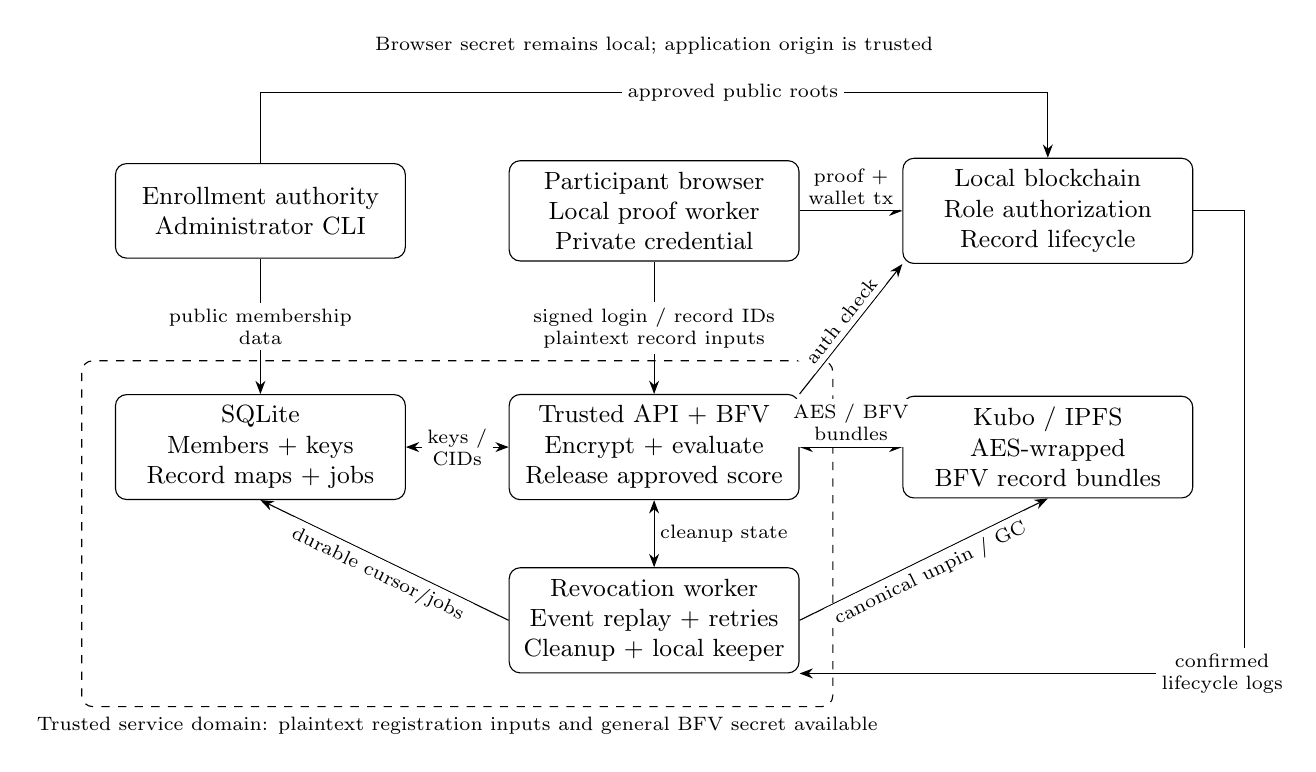
\begin{tikzpicture}[
  >=Stealth,
  box/.style={draw,rounded corners,align=center,text width=3.4cm,minimum height=1.2cm,inner sep=4pt,font={\small\hyphenpenalty=10000\exhyphenpenalty=10000},fill=white},
  labeltext/.style={font=\scriptsize,align=center,fill=white,inner sep=2pt}]
\node[box] (admin) at (0,3) {Enrollment authority\\Administrator CLI};
\node[box] (browser) at (5,3) {Participant browser\\Local proof worker\\Private credential};
\node[box] (chain) at (10,3) {Local blockchain\\Role authorization\\Record lifecycle};
\node[box] (db) at (0,0) {SQLite\\Members + keys\\Record maps + jobs};
\node[box] (api) at (5,0) {Trusted API + BFV\\Encrypt + evaluate\\Release approved score};
\node[box] (ipfs) at (10,0) {Kubo / IPFS\\AES-wrapped\\BFV record bundles};
\node[box] (worker) at (5,-2.2) {Revocation worker\\Event replay + retries\\Cleanup + local keeper};
\begin{pgfonlayer}{background}
\node[draw,dashed,rounded corners,fit=(db)(api)(worker),inner sep=12pt,
  label={[font=\scriptsize]below:Trusted service domain: plaintext registration inputs and general BFV secret available}] {};
\end{pgfonlayer}
\draw[->] (admin.north) -- ++(0,0.9) -| node[pos=.3,labeltext] {approved public roots} (chain.north);
\draw[->] (admin) -- node[labeltext] {public membership\\data} (db);
\draw[->] (browser) -- node[labeltext] {signed login / record IDs\\plaintext record inputs} (api);
\draw[->] (browser) -- node[above,labeltext] {proof +\\wallet tx} (chain);
\draw[<->] (api) -- node[labeltext] {keys /\\CIDs} (db);
\draw[<->] (api) -- node[above,labeltext] {AES / BFV\\bundles} (ipfs);
\draw[->] (api.north east) -- node[above,sloped,labeltext] {auth check} (chain.south west);
\draw[<->] (api) -- node[right,labeltext] {cleanup state} (worker);
\draw[->] (worker.west) -- node[below,sloped,labeltext] {durable cursor/jobs} (db.south);
\draw[->] (worker.east) -- node[below,sloped,labeltext] {canonical unpin / GC} (ipfs.south);
\draw[->] (chain.east) -- ++(0.65,0) |- node[pos=.6,right,labeltext] {confirmed\\lifecycle logs} (worker.south east);
\node[font=\scriptsize,align=center] at (5,5.1) {Browser secret remains local; application origin is trusted};
\end{tikzpicture}%
}

\caption{Implemented architecture. The dashed box marks the trusted service domain. Administrative signing is separate; browser secrets remain local, while record-registration inputs are visible to the trusted service. Public-chain and storage visibility are explicitly different.}
\label{fig:architecture}
\end{figure*}

\subsection{Enrollment and Local Credential Handling}
The browser samples a 248-bit random field-compatible secret $s$ and exports a
credential JSON file. For role $r\in\{0,\ldots,5\}$, the public leaf is
\begin{equation}
 L=H(s,r),
 \label{eq:leaf}
\end{equation}
where $H$ is the circomlib-compatible two-input Poseidon hash. A local administrator
approves $L$ in a persistent depth-20 role tree and publishes its root. Login only
reads existing membership data; it cannot enroll a caller or modify a root.

The leaf is a public commitment, not a password. The private credential secret is
the sensitive authenticator. Importing the JSON file reads it with the browser's
File API; the file is not uploaded to the backend. The secret and Merkle witness
are passed to an in-browser worker. Copying a leaf alone does not provide the
corresponding witness. A stolen credential file, however, is a serious compromise;
the approved leaf is not permanently bound to one enrollment wallet.

Root updates increment a version and invalidate earlier sessions for that role.
Credential removal requires administrator approval of an updated tree. A staged
membership update that fails on-chain remains visibly inconsistent until the
administrator reconciles it; the API does not silently serve a mismatching root.

\subsection{Proof Binding and On-Chain Authorization}
Private circuit inputs comprise the secret, fresh salt $\rho$, twenty sibling
hashes and twenty path selectors. Selectors satisfy $b(b-1)=0$. The public signal
order is root, role, nullifier, wallet, chain ID, issuer and root version. Using
$a,c,k,v$ for wallet, chain, issuer and version, respectively,
\begin{equation}
 n=H\!\left(s,H\!\left(\rho,H\!\left(a,H\!\left(c,H(k,v)\right)\right)\right)\right).
 \label{eq:nullifier}
\end{equation}

The contract checks role consistency, current root/version, recipient equal to
\code{msg.sender}, chain and issuer domain, unused nullifier and the Groth16
pairing relation. A valid proof creates a four-hour authorization session.
\code{PFEKeyIssuer} is a retained historical contract name: this function issues
authorization state, not an FE decryption key.

The compiled BN254/\code{bn-128} circuit has 13,513 R1CS constraints, 42 private
inputs and seven public inputs. This replaces the old report's 5,391-constraint,
four-public-input description. A genuine secret phase-two contribution is included
and the final key is verified against the R1CS and prepared power-14 transcript.
The phase-one transcript is inherited locally and phase two has one local
contributor; no independent multiparty setup is claimed.

\subsection{Wallet Connection, API Session and Role Policy}
Connecting the wallet checks its selected chain and requests an explicit network
switch when needed. The browser verifies the result before showing a connected
account. Account or network changes clear credentials, session state and results.
These usability checks complement, rather than replace, contract domain checks.

After on-chain authorization, the API issues a five-minute single-use challenge
containing the origin, wallet, chain, issuer, nonce and expiry. The wallet signs it
to establish a random bearer session. Only a digest of the bearer token is stored;
its expiry cannot exceed the on-chain authorization. Every protected request checks
current role, expiry and root version. An owner or subject can revoke an on-chain
session; preventing future authentication also requires removal of its credential.

\begin{table}[t]
\centering\scriptsize
\caption{Implemented role permissions. D/R denote donor/recipient registration; M denotes matching and V record revocation.}
\label{tab:roles}
\renewcommand{\arraystretch}{1.12}
\begin{tabularx}{\columnwidth}{Xrrrrrr}
\toprule Role & ID & Mask & D & R & M & V\\\midrule
Doctor & 0 & 7 & Y & Y & Y & N\\
Coordinator & 1 & 7 & Y & Y & Y & N\\
Procurement & 2 & 3 & Y & N & Y & N\\
Matching & 3 & 1 & N & N & Y & N\\
Transporter & 4 & 0 & N & N & N & N\\
Surgeon & 5 & 9 & N & N & Y & Y\\\bottomrule
\end{tabularx}
\end{table}

Permission bits are matching~0, donor registration~1, recipient registration~2
and revocation~3. Table~\ref{tab:roles} is enforced in contracts, APIs and the UI.
Administrative enrollment and retention scheduling are separate. No transport or
transplant permission is claimed without an implemented workflow.

\subsection{Encrypted Record Storage and Registration}
Each record contains two ABO flags, six binary synthetic tissue features and
urgency: nine BFV ciphertexts. Parameters are polynomial degree 4096,
\code{BFVDefault} coefficient moduli selected for SEAL's \code{tc128} validation
and a 20-bit batching plaintext modulus, $t=1{,}032{,}193$. Each scalar attribute
is replicated across all 4096 batching slots; result release reads the first slot.
Different pairs are not packed into separate SIMD slots in this revision. Integers
are represented directly, without floating-point or fixed-point scaling. Evaluated ciphertexts must retain a positive
noise budget and decrypted results must satisfy the specified bounds.

The BFV bundle is wrapped using a fresh AES-256-GCM data key and record-ID
authenticated context before upload to IPFS. The BFV secret and individual record
keys are encrypted at rest under an operator-provided 32-byte wrapping secret.
SQLite records the key version, wrapped record key and canonical CID. Missing or
incorrect key material causes explicit failure. Existing on-chain records also
prevent startup with an empty replacement key database.

Registration has three steps: the authorized service prepares encrypted storage;
the participant wallet registers the opaque record ID, encrypted-content anchor
and entity type; the service confirms the canonical owner, type, activity and anchor.
The anchor is \code{keccak256} of the canonical CID. Neither the CID itself nor
plaintext ABO, tissue features or urgency appears in revised contract inputs,
storage or events. Pending registrations can be retried after wallet failure;
abandoned uploads require operator retention review.

\subsection{Fixed Homomorphic Eligibility and Ranking}
The ordinary synthetic ABO policy permits O to all groups, A to A/AB, B to B/AB
and AB to AB. It is a demonstration policy, not a complete transplant-eligibility
rule. Rh and incompatible-transplant exceptions are excluded.
With donor/recipient antigen flags $A_D,B_D,A_R,B_R$, BFV evaluates
\begin{equation}
 I=A_D(1-A_R)+B_D(1-B_R).
 \label{eq:eligibility}
\end{equation}
Only $I=0$ is eligible. Ineligible pairs have no score and are displayed as
``Ineligible under demo policy.''

\begin{table}[t]
\centering\scriptsize
\caption{Synthetic ABO encoding and ordinary demo eligibility. Entries are recipient ABO groups, not Rh types.}
\label{tab:abo}
\begin{tabular}{lcc}\toprule Donor ABO & $(A_D,B_D)$ & Eligible recipients\\\midrule
O & $(0,0)$ & O, A, B, AB\\
A & $(1,0)$ & A, AB\\
B & $(0,1)$ & B, AB\\
AB & $(1,1)$ & AB\\\bottomrule
\end{tabular}
\end{table}

For six binary toy tissue features, define the mismatch count and fixed numerator
as follows:
\begin{align}
 m&=\sum_{j=1}^{6}(d_j-r_j)^2,\label{eq:mismatch}\\
 N&=4200-700m+900u,\label{eq:numerator}\\
 S&=\operatorname{round}(N/6),\quad u\in\{0,1,2\}.\label{eq:score}
\end{align}
Here $u$ is recipient urgency. Donor urgency has no ranking effect. BFV evaluates
$I$ and $N$; only after approved decryption does the service divide by six and
round. For eligible pairs, $0\leq m\leq6$, $0\leq N\leq6000$ and $0\leq S\leq1000$.
The features are not clinical HLA typing, and weights 700/150 are experimental.
Scores are synthetic ranking points, not compatibility percentages.

Matching accepts only canonical donor/recipient IDs. Clients cannot select a
ciphertext, function, weight or decryption target. Batch jobs allow at most ten
distinct IDs on each side and release results only to their owner. Jobs cache
encrypted BFV bundles within the job, recheck authorization and record activity,
sort eligible scores descending and break ties by donor then recipient ID. Ranking
does not reserve organs or compute an optimal assignment.

\subsection{Recoverable Record Revocation}
The Surgeon requests and executes revocation by opaque record ID for either entity
type. Confirmed chain deactivation immediately blocks new matching independently
of cleanup progress. The caller cannot supply a CID for cleanup.

A durable worker replays ordered logs from its persisted cursor, resolves canonical
records, removes the service-held wrapped data key, unpins the local CID and runs
local garbage collection. Confirmation depth defaults to one locally and six for a
later public-testnet experiment. Block/hash/log metadata and retry state survive
process restarts. A detected change to processed history halts destructive work for
operator audit because key deletion cannot be rolled back.

States distinguish requested, deactivated, cleanup pending, completed locally and
failed. Failures retry with bounded exponential backoff capped at one hour, and an
administrator can queue another attempt. Retention schedules are processed through
a cursor inspecting at most fifty entries per call; a local keeper submits that
permissionless processing operation. Application ranking jobs interrupted by restart
are marked failed and resubmitted, whereas cleanup jobs recover from persistent state.

\section{Implementation and Evaluation}
\label{sec:impl}

\subsection{Technology Stack and Reproducibility}
Table~\ref{tab:stack} gives the evaluated software versions. The source of truth for
model and protocol behavior is \code{docs/PROTOCOL\_V2.md}. This report separates
the measured 22~October benchmark from subsequent UI/network-handling fixes and
the 23~October regression run. Historical root-level benchmark files are not mixed
with the revised measurements.

\begin{table}[t]
\centering\scriptsize\renewcommand{\arraystretch}{1.1}
\caption{Evaluated implementation stack.}
\label{tab:stack}
\begin{tabularx}{\columnwidth}{>{\raggedright\arraybackslash}p{1.65cm} >{\raggedright\arraybackslash}X}
\toprule Component & Technology/version\\\midrule
Local EVM & Hardhat 2.29.1; chain 31337; Solidity 0.8.20\\
ZKP & circom 2.2.3; snarkjs 0.7.6; Groth16/BN254\\
Hash/tree & Poseidon, depth 20, persistent multi-member role trees\\
HE & node-seal 5.1.7, BFV, degree 4096\\
Backend & Node 22.19.0; Express 4.22.3; built-in SQLite\\
Frontend & React 19.2.8; Vite 8.2.2; ethers 6.17.0\\
Storage & Kubo 0.33.2; native Node fetch/FormData adapter\\
Testing & Hardhat/Chai; Playwright with installed Edge\\\bottomrule
\end{tabularx}
\end{table}

The benchmark machine is an Intel Core i7-12700H with approximately 16\,GB RAM,
Windows and Node 22.19.0. Raw samples include dependency versions, OS/architecture,
hardware, the parent commit, dirty-working-tree status, source hashes and
circuit/key hashes. The parent commit is
\code{5edd45f2a6f5abff6b65992a04a4e1c41cf0933a}; it is the historical parent, not a
claim that the revised working tree was committed. Full identifiers are supplied
in the accompanying evidence files.
The evaluated Kubo daemon runs offline in an isolated local repository; these
experiments do not measure peer-to-peer replication or remote retrieval.

\subsection{Validation Evidence and Test Boundaries}
The archived complete validation passed 28 tests with zero skips, including one
live browser/API/Kubo/Hardhat integration test. That demonstration contains eleven
checks covering unapproved membership rejection, local proof generation,
registration, retrieved-record matching, restart persistence, batch ranking, donor
cleanup, recipient revocation during downtime, Transporter restrictions,
missing-key failure and absence of credential secrets in captured API request bodies.
It uses an EIP-1193 development-wallet adapter, not automated interaction with the
MetaMask extension.

After the network-selection UI fixes, the 23~October default regression passed
\CurrentTestsPassed{} tests, with \CurrentTestsSkipped{} explicit skip for the
infrastructure integration test. Eight wallet-network cases cover selected-chain
checking, switch/add behavior, rejected or pending prompts and failure to switch.
A separate headless browser check exercises six network/credential-reset assertions
with a simulated provider. These counts describe separate runs; they are not added
together as a single test total. A fresh live run of the final UI and systematic
manual MetaMask sign-off remain necessary for release verification.

Arithmetic tests cover all 16 ABO pairs across three urgency classes, every
mismatch count from zero to six across all urgency classes, and twenty seeded
synthetic cases compared with independent plaintext calculations. They check
positive BFV noise budgets, persistent-key recovery and malformed input rejection.
The seeded cases supplement, rather than replace, the explicit boundary matrix;
they are not statistical evidence about a clinical population.

Contract/API tests cover roles, domain binding, public-signal tampering, nullifier
replay, expiry, explicit revocation, root changes, job ownership and removed unsafe
routes. Recovery fault-injection tests cover offline catch-up, GC failure, retries,
confirmation depth and processed-history changes. No numerical source-code coverage
percentage or formal end-to-end security proof is asserted.

\subsection{Experiment Design}
Repeated timing experiments use ten warmups and thirty measured repetitions.
Tables report empirical upper-middle medians, nearest-rank p95 and population
standard deviation (SD); raw samples are retained. Enrollment measures adding
members to a progressively growing approved tree. Proving time is Node snarkjs
execution including witness/path preparation, not a browser latency measurement.
Initial authorization gas is recorded separately from warmed updates of an existing
wallet session. Dataset-registration gas has twenty samples; repeated gas/timing
series have thirty measured samples.

The same authenticated HTTP job interface evaluates $1\times1$, $5\times5$ and
$10\times10$ workloads for plaintext wallet RBAC, BFV wallet RBAC and BFV ZKP
authorization. Each configuration uses an established session; a fresh proof is not
generated per pair or job. The plaintext baseline holds attributes in memory,
whereas BFV retrieves real AES-wrapped Kubo records. Thus differences include
storage/protection costs and cannot isolate cryptography alone.

Workload donors have ABO~O and features $(1,0,1,0,1,0)$; recipients have ABO~A and
features $(1,1,1,0,0,0)$, with urgency cycling through zero, one and two. All pairs
are eligible and have two mismatches. Opaque IDs are fresh. This fixed fixture
exercises score release; randomized and ineligible cases are separate correctness
tests.

HTTP timings include job submission and 100-ms result polling using fresh
connections. Bounded retries are permitted only for idempotent polling transport
failures and remain in measured time; the completed run recorded zero retries.
Benchmark-only request quotas are raised to permit repetitions. The normal API
retains its limits: one active job per wallet, 200 submitted pairs per fifteen
minutes and twenty pending records per wallet.

\subsection{Measured Timing and Gas Results}
\begin{table}[t]
\centering\scriptsize
\caption{Stage timing in milliseconds: 10 warmups and 30 measured samples per row. SD is population standard deviation.}
\label{tab:timings}
\setlength{\tabcolsep}{3pt}\renewcommand{\arraystretch}{1.1}
\begin{tabularx}{\columnwidth}{>{\raggedright\arraybackslash}Xrrr}
\toprule Stage & Median & p95 & SD\\\midrule
Approved-root enrollment & 38.58 & 45.93 & 4.69\\
Membership witness & 47.82 & 50.29 & 1.01\\
Node proof generation & 2,922.25 & 4,318.04 & 1,168.12\\
Local authorization receipt & 10.45 & 11.76 & 0.86\\
BFV record encryption & 115.16 & 131.60 & 8.89\\
BFV policy evaluation & 230.73 & 244.98 & 7.60\\
Permitted-result release & 10.47 & 16.85 & 2.76\\
Wallet-signature check & 10.25 & 13.00 & 1.37\\
Encrypted storage retrieval & 42.03 & 107.35 & 20.37\\
Local revocation request & 1.87 & 2.41 & 4.94\\
Local deactivation receipt & 1.66 & 2.07 & 0.23\\
Direct local cleanup & 22.62 & 31.28 & 5.13\\
\bottomrule\end{tabularx}
\end{table}

\begin{table}[t]
\centering\scriptsize
\caption{Gas used: medians for repeated series, individual gas for one-sample rows.}
\label{tab:gas}
\setlength{\tabcolsep}{3pt}\renewcommand{\arraystretch}{1.1}
\begin{tabularx}{\columnwidth}{>{\raggedright\arraybackslash}Xrr}
\toprule Operation & Gas & Samples\\\midrule
Wallet-RBAC enrollment (baseline) & 43,928 & 1\\
Role-root update & 36,537 & 30\\
First wallet authorization & 367,339 & 1\\
Warmed reauthorization & 310,463 & 30\\
One record registration & 110,259 & 20\\
Revocation request & 69,513 & 30\\
Revocation execution & 58,717 & 30\\
\bottomrule\end{tabularx}
\par\smallskip\raggedright First enrollment of an empty role, deployment, session revocation and retention scheduling/keeper gas were not separately measured. Off-chain stages incur no chain transaction gas.
\end{table}

\begin{table*}[t]
\centering\scriptsize
\caption{Authenticated HTTP matching-job latency in milliseconds: 10 warmups and 30 measured samples per configuration. Jobs use established sessions and include 100-ms result polling.}
\label{tab:workloads}
\renewcommand{\arraystretch}{1.12}
\begin{tabularx}{\textwidth}{>{\raggedright\arraybackslash}Xlrrr}
\toprule Configuration & Matrix & Median & p95 & SD\\\midrule
Plaintext + wallet RBAC & $1\times1$ & 134.88 & 146.71 & 6.54\\
Plaintext + wallet RBAC & $5\times5$ & 291.90 & 336.71 & 47.04\\
Plaintext + wallet RBAC & $10\times10$ & 862.31 & 1,080.33 & 72.85\\
BFV + wallet RBAC & $1\times1$ & 384.68 & 599.39 & 85.15\\
BFV + wallet RBAC & $5\times5$ & 7,203.02 & 7,486.88 & 173.74\\
BFV + wallet RBAC & $10\times10$ & 11,946.91 & 17,289.18 & 1,464.74\\
BFV + ZKP authorization & $1\times1$ & 164.48 & 198.90 & 11.34\\
BFV + ZKP authorization & $5\times5$ & 3,292.05 & 3,423.10 & 77.39\\
BFV + ZKP authorization & $10\times10$ & 12,116.84 & 12,406.25 & 148.14\\
\bottomrule\end{tabularx}
\end{table*}


The median Node proving time is \ProofMedianMs{}\,ms and median BFV evaluation is
\EvaluationMedianMs{}\,ms (Table~\ref{tab:timings}). Proving variation is substantial
and must be retained in interpretation. Gas costs (Table~\ref{tab:gas}) distinguish
first authorization from warmed reauthorization and separate revocation request
from execution. Credential import, browser proving, wallet-message signing,
off-chain evaluation, storage and local cleanup do not themselves submit chain
transactions. Zero chain gas does not mean zero compute or storage cost.

Figure~\ref{fig:workload} and Table~\ref{tab:workloads} report completed workload
measurements. Baselines execute sequentially in a fixed order on one machine.
Thermal state, host load and order effects are not controlled; these descriptive
statistics do not establish a causal ZKP speedup or slowdown. In particular, the
small-workload gap between the two BFV configurations must not be attributed to
proof verification, since proof issuance is not part of each job. Variation between
microbenchmarks and later HTTP runs further limits cross-stage extrapolation.

\begin{figure*}[t]
\centering
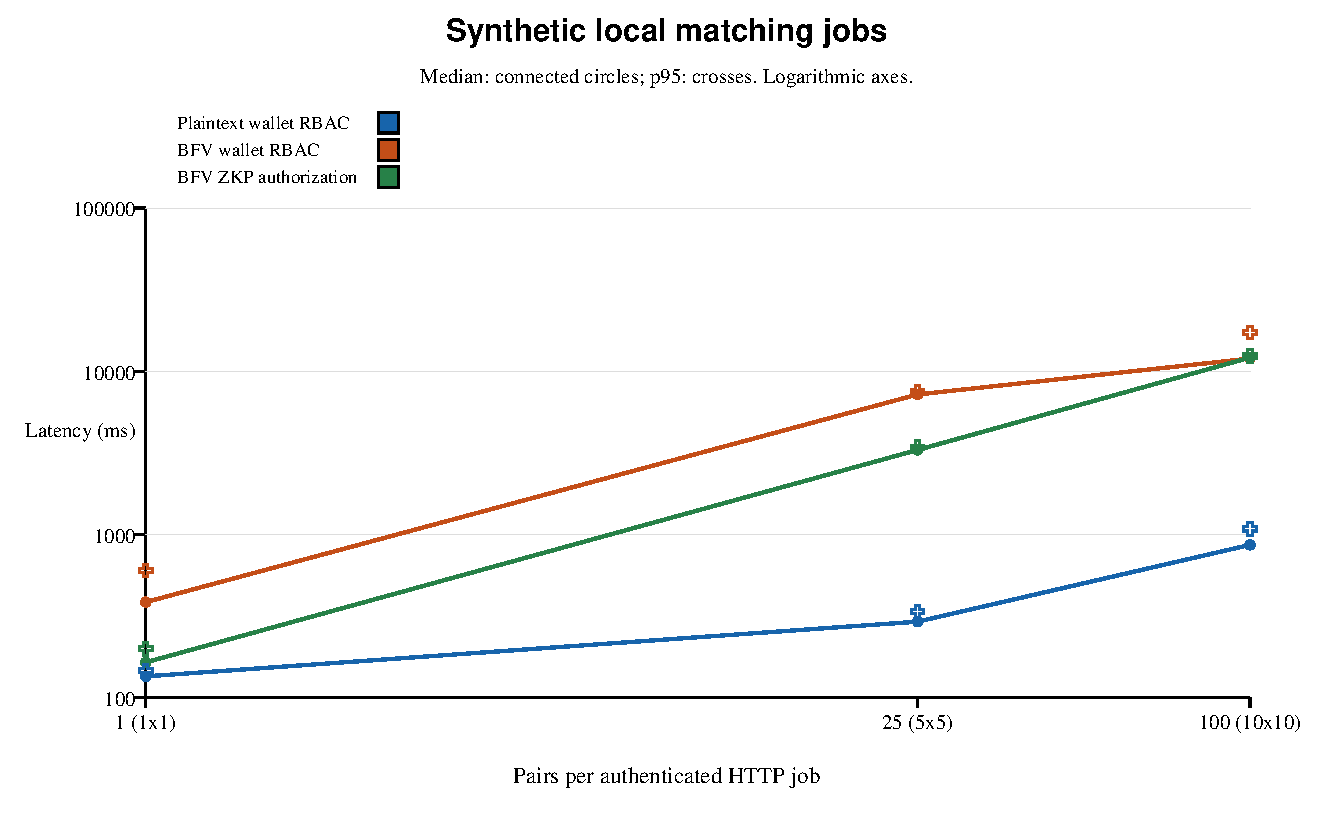
\includegraphics[width=0.86\textwidth]{figures/workload-latency.pdf}
\caption{Local authenticated synthetic matching jobs. Connected circles show medians; crosses show p95. Both axes are logarithmic. Fixed-order execution, storage differences and polling overhead limit causal comparison.}
\label{fig:workload}
\end{figure*}

Revocation timings isolate local request receipts, execution receipts and direct
key deletion/unpin/GC. Donor and recipient records alternate across repetitions.
Direct cleanup excludes the worker's discovery interval, confirmation wait and
retry delay; it is not total user-observed erasure time. The local EVM also excludes
public-network consensus and finality costs.

\subsection{Research-Question Assessment}
\textbf{RQ1:} The recorded adversarial cases enforce the specified role/session
policy under trusted enrollment. They do not establish correctness of real-world
institutional identity checks.

\textbf{RQ2:} Proof generation, initial/warmed authorization and authenticated
workloads have separate measured costs. Login costs are amortized over a session;
the fixed-order workload experiment supports descriptive results rather than a
causal estimate of small differences between BFV baselines.

\textbf{RQ3:} Encrypted and plaintext calculations agree across the implemented
ABO matrix, boundary set and seeded fixtures. This establishes arithmetic
correctness for the synthetic model, not clinical suitability.

\textbf{RQ4:} Recorded tests recover persistent records, replay missed revocation
events and expose retryable cleanup failure. Interrupted ranking jobs require
resubmission. Deep-history changes halt irreversible work for operator audit.

\section{Security Analysis}
\label{sec:security}

\subsection{Proof Soundness, Enrollment and Credential Secrecy}
The proof statement concerns knowledge of a secret that yields an approved leaf
and valid Merkle path. Boolean selector and role constraints prevent malformed
witness selection. Groth16 security also depends on its assumptions and setup;
verification of a transcript is not a replacement for an independent ceremony.
The enrollment authority remains responsible for approving the right participant.

The normal import/authentication flow does not transmit the credential secret.
Only a proof/public signals, a wallet transaction and a signed API challenge leave
the browser. Nevertheless, a malicious frontend origin or privileged extension
could exfiltrate local secrets. Browser-local proving does not protect a compromised
endpoint, and the exported JSON file requires private backup and handling.

\subsection{Replay, Domain Binding and Session Control}
A copied proof cannot authorize another recipient because its public wallet and
\code{msg.sender} must agree. Chain, issuer and root-version checks restrict its
domain; used nullifiers reject identical resubmission. A credential holder can
produce fresh proofs with fresh salt, so session revocation alone does not remove
membership. Credential removal and root publication are the mechanisms that prevent
later proofs from the removed secret.

Wallet-signed challenges are single-use and expire after five minutes. API tokens
have bounded lifetimes and current authorization is checked per operation and
before result release. Cached ciphertexts do not bypass activity checks. Bearer
tokens remain sensitive while valid; local loopback HTTP is the evaluated transport,
and a remote deployment would require protected transport and operational review.

\subsection{Storage Confidentiality, Integrity and Output Leakage}
AES-GCM protects stored bundles under the retained record key, while the chain
anchor binds the canonical encrypted content. A general BFV secret remains in the
trusted-service domain. An adversary compromising that service can access inputs,
available keys and plaintext results; these are explicit limits of the design.

The API forbids arbitrary ciphertext decryption, caller-selected evaluation
functions and direct unpin targets. This reduces its exposed interface but does
not make it FE or eliminate inference. Eligible scores and repeated chosen-record
queries may reveal relationships between features. Quotas and fixed output formats
are operational restrictions, not a formal leakage bound or differential-privacy
guarantee. Wallets and lifecycle metadata remain linkable.

\subsection{Retention Controls and GDPR Boundaries}
IPFS persistence depends on holders of copies; local unpinning does not recall
external replicas~\cite{ipfs}. Removing the live service-held data key cannot erase
backups, copied keys, previously decrypted bundles or released scores. The chain
continues to retain audit metadata. Cleanup status is an operator/service report,
not a cryptographic proof that every replica was destroyed.

The implementation demonstrates access deactivation and defined local cleanup.
It does not establish GDPR compliance or fulfillment of every erasure request.
The GDPR includes data minimisation in Article~5(1)(c) and erasure rights with
conditions/exceptions in Article~17~\cite{gdpr}. Any actual deployment would require
an applicable lawful basis, a retention/backup policy and an assessment of what
remaining identifiers and copies mean for the particular processing context.

\subsection{Remaining Operational and Experimental Limits}
The system has one trusted decryption service and local SQLite key custody,
without HSM isolation or multi-hospital key governance. Pending unregistered uploads
need operator review. Dependency checks recorded zero high/critical and two moderate
production advisories; this is not a complete security audit. The current stack
does not claim post-quantum security. A local chain and test-wallet adapter do not
establish permissioned-consortium behavior, public-network finality or complete
MetaMask-extension compatibility.

\section{Conclusion and Future Work}
\label{sec:conclusion}
This Phase~II prototype integrates approved role membership, browser-generated
proofs, fixed BFV matching, encrypted off-chain records and recoverable local
revocation. The revised account of its behavior distinguishes authorization from
FE key issuance, arithmetic correctness from clinical validity and local cleanup
from universal erasure. Recorded correctness/recovery tests and raw measurements
provide evidence for the four research questions under the stated trust assumptions.

Near-term work is to complete a fresh final-UI browser run and manual MetaMask
check, obtain independent setup contributions, review dependency/retention handling
and repeat workload experiments with counterbalanced ordering. Clinical eligibility
and allocation rules need domain-expert validation before any patient-data use.
Stronger key custody, multi-institution governance, actual functional encryption
and post-quantum migration each require separate design and evaluation. Public
deployment awaits operational and governance review.

\begingroup
\small\raggedright
\newcommand{\BIBdecl}{\setlength{\itemsep}{0pt}\setlength{\parsep}{0pt}\setlength{\parskip}{0pt}}
\bibliographystyle{IEEEtran}
\bibliography{references}
\endgroup
\end{document}
